\documentclass[letterpaper,addpoints, 11pt]{exam}

\usepackage{graphicx}  
\usepackage{amsmath, latexsym, color, graphicx, amssymb, bm, here, enumerate}
\usepackage{epsf, epsfig, pifont,tikz,subfigure}
\usepackage{graphics, calrsfs}
\usepackage{times}
\usepackage{fancybox,calc}
\usepackage{palatino,mathpazo}
\usepackage{amsfonts}
\usepackage{wrapfig}
\usepackage{multicol}
\usepackage{sidecap}
\usepackage{hyperref}
\usepackage{media9}
\usepackage{mathtools}
\usepackage{soul}
\usepackage{enumitem}
\usepackage[margin=0.5in, footskip=0.25in]{geometry}
\usepackage{sectsty}
\sectionfont{\centering}
\renewcommand\thesection{\Roman{section}.}
\renewcommand\thesubsection{\Alph{subsection}.}
\renewcommand\thesubsubsection{\thesubsection \arabic{subsubsection}.}
\usepackage{listings}
\usepackage{caption}
\DeclareCaptionFont{white}{\color{white}}
\DeclareCaptionFormat{listing}{%
	\parbox{\textwidth}{\colorbox{gray}{\parbox{\textwidth}{#1#2#3}}\vskip-4pt}}
\captionsetup[lstlisting]{format=listing,labelfont=white,textfont=white}
\lstset{frame=lrb,xleftmargin=\fboxsep,xrightmargin=-\fboxsep}
\usepackage{url}
\urlstyle{same}
\usepackage{wasysym}
\usepackage[export]{adjustbox}
%_______________________________________________



\begin{document}

\begin{center}
	\Large \textbf{ISA 401/501 - Business Intelligence \& Data Viz} \\
	\Large \textbf{14: An Overview of Data Viz Software} \\
\end{center}

%\vspace{5mm}
%
%\makebox[\textwidth]{Name and ID:\enspace\hrulefill}
%
%\vspace{5mm}
%
%\makebox[\textwidth]{Section:\enspace\hrulefill}

\begin{center}
	\fbox{\fbox{\parbox{\textwidth}{\centering
				\textbf{\large Learning Objectives for Today's Class:}
				\vspace{-2mm}
				\begin{enumerate}[label=(\Alph*)]
					\item Constructing simple visualizations using \textbf{Power BI}
					\begin{itemize}[nosep]
						\item Connecting to data using Power BI and understanding its basic terminology. 
						\item The ETL Process in Power BI. 
						\item Creating simple visualizations with filters in Power BI.
					\end{itemize}
					\item Creating a Storyboard Using \textbf{Tableau}
					
				\end{enumerate}
			}}}
		\end{center}	
%		\begin{center}
%			\addpoints
%			\combinedgradetable[h][questions]
%		\end{center}
%		
%		\newpage

\begin{questions}

\question[0] As an illustrative example of some of the features of \textbf{Power BI}, we will be using the BTS flight delay dataset (from: \url{https://www.transtats.bts.gov/DL_SelectFields.aspx?gnoyr_VQ=FGK&QO_fu146_anzr=b0-gvzr}). For your convenience, I extracted the data for June-July of 2022, and  added the airline abbreviation lookup CSV file. The links to these files are on \underline{Canvas} under Week 08. As we will go through the demonstration, you are encouraged to note the following: 
\begin{enumerate}[label=(\Alph*)]
	\item How to use the ``Get Data" button and the ``Query Editor" to \textbf{extract} the 2 months of data into Power BI. \textbf{Note how Power BI automatically classifies/``guesses" the data types}.\\
	\bigskip \bigskip \bigskip \bigskip
	
	\noindent \underline{\textbf{Some Transformation Steps:}}
	\item How to append the data from June--July. into one table.
	\bigskip \bigskip \bigskip  
	\item Import and merge the CSV file to the generated table. \textbf{Note how we will also involve fixing the issue that this imported column may not read the column titles.}
	\bigskip \bigskip
	\item Minor: how to move the ``location of the added column" in the ``Query Editor"
	\bigskip
	\item Let us make the table more manageable by only selecting: 
	\begin{itemize}[nosep]
		\item MONTH
		\item FL\_DATE
		\item Airline
		\item FL\_NUM
		\item ORIGIN\_CITY\_NAME
		\item DEST\_CITY\_NAME
		\item DEP\_DELAY 
		\item ARR\_DELAY
	\end{itemize}
	\item Let us ensure that the data types are appropriate and then \textbf{load} the data into Power BI.
	\bigskip \bigskip
	\item \textbf{Let us create a similar visualization; note that the numbers would be different since the data shown below is not from 2021.}	
\end{enumerate}
 	
{\centering 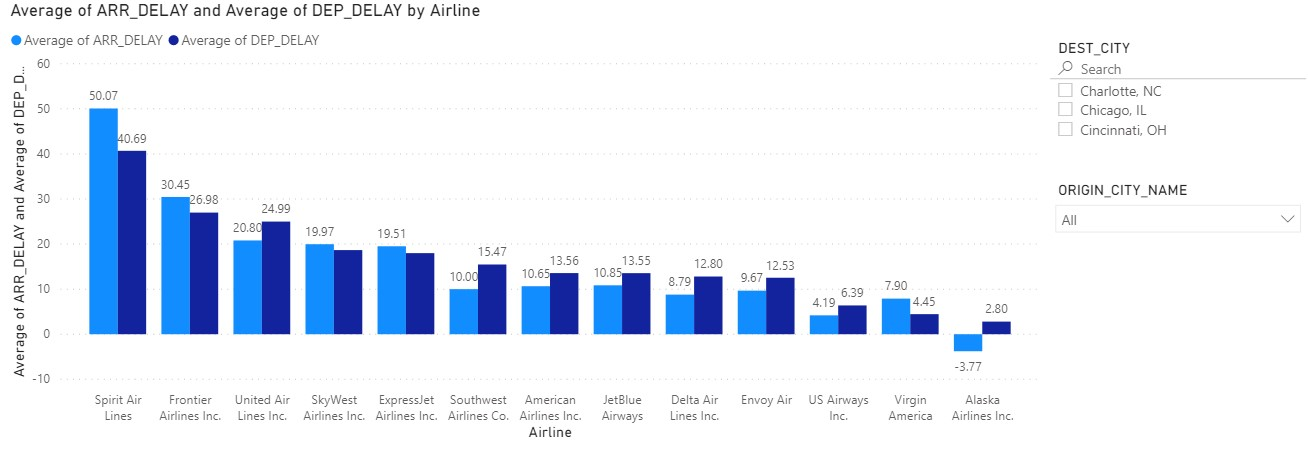
\includegraphics[width=\textwidth,frame]{figures/powerbi}}

\vspace{0.25in}



\end{questions}
\end{document}
